\question 在以下磁盘调度算法中,可能出现饥饿现象的是
\par\twoch{电梯调度}{\textcolor{red}{最短寻道时间优先}}{循环扫描算法}{先来先服务}
\begin{solution}最短寻道时间优先(SSTF)调度算法基本上是一种最短作业优先(SJF)调度,和SJF一样,它可能导致一些请求得不到服务,即出现饥饿现象。
\end{solution}
\question 设磁盘的I/O请求队列中的柱面号为55、58、39、18、90、160、150、38、184,磁头的起始位置为100,若采用SSTF(最短寻道时间优先)算法,则磁头需移动的磁道数为
\par\twoch{55}{184}{200}{\textcolor{red}{248}}
\begin{solution}对于SSTF算法,寻道顺序为100、90、58、55、39、38、18、150、160、184,移动磁道次数分别为10、32、3、16、1、20、132、10、24,总数为248。
\end{solution}
\question (河北大学,2005年)系统中磁头停留在磁道号为70的磁盘上,这时先后有4个进程提出了磁盘访问请求,要访问的磁盘的磁道号按申请到达的先后顺序依次为40,60,20,90。移动臂的运动方向沿磁道号递增的方向移动。若采用SCAN算法,所需寻道长度(走过多少柱面)为
\par\twoch{100}{\textcolor{red}{90}}{120}{以上都不同}
\begin{solution}磁道访问序列为:70→90→60→40→20,移动臂的运动方向先沿磁道号递增的方向移动,等磁道号递增方向没有请求了(响应90的请求后),开始向磁道号递减方向移动(依次响应60、40、20)。
总共所需寻道长度=20+30+20+20=90,因此本题选B。
\end{solution}
\question 假设磁头当前位于第105道,正在向磁道序号增加的方向移动。现有一个磁道访问请求序列为35,45,12,68,110,180
,170,195,采用SCAN调度(电梯调度)算法得到的磁道访问序列是( )
\par\fourch{\textcolor{red}{110,170,180,195,68,45,35,12}}{110,68,45,35,12,170,180,195}{110,170,180,195,12,35,45,68}{12,35,45,68,110,170,180,195}
\begin{solution}SCAN算法的基本思想:磁头从磁盘的一端开始向另一端移动,沿途响应访问请求,直到到达了磁盘的另一端,此时磁头反方向移动并继续响应服务请求,其运动轨迹类似于电梯一上一下的运行。根据题目条件,磁头向磁道序号增加方向移动,第一个响应的请求是110磁道,排除D选项,然后继续朝着增大的方向移动,响应170、180、195,因此排除B选项,然后从磁道最大开始,向磁道最低移动,依次响应68、45、35、12,排除C。因此可以得到访问序列是A。
【总结】
本题画图也可以很好地解答(见下图),把请求序列依据磁道大小画在对应位置,然后按照SCAN算法的移动方向扫描,就得到了答案,可以作为检验手段。
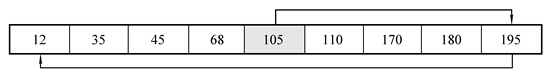
\includegraphics[width=5.73958in,height=0.81250in]{computerassets/8b7f43b8e182f4cc4665922fbe7c606c.jpeg}
\end{solution}
